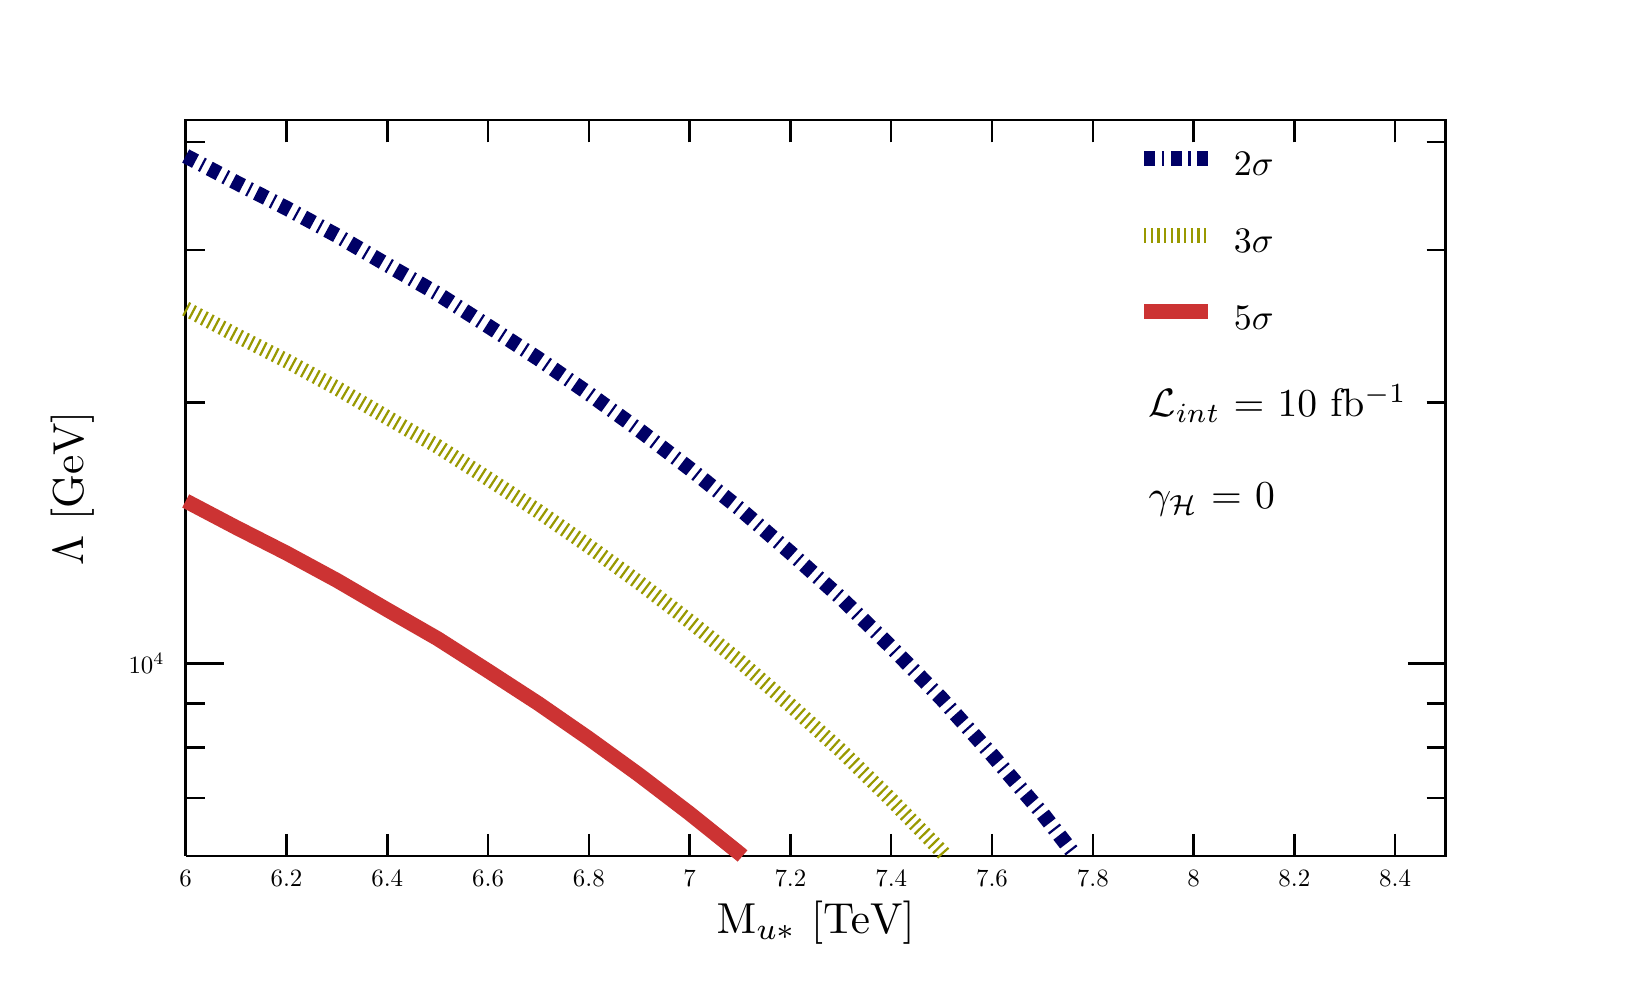
\begin{tikzpicture}
\pgfdeclareplotmark{cross} {
\pgfpathmoveto{\pgfpoint{-0.3\pgfplotmarksize}{\pgfplotmarksize}}
\pgfpathlineto{\pgfpoint{+0.3\pgfplotmarksize}{\pgfplotmarksize}}
\pgfpathlineto{\pgfpoint{+0.3\pgfplotmarksize}{0.3\pgfplotmarksize}}
\pgfpathlineto{\pgfpoint{+1\pgfplotmarksize}{0.3\pgfplotmarksize}}
\pgfpathlineto{\pgfpoint{+1\pgfplotmarksize}{-0.3\pgfplotmarksize}}
\pgfpathlineto{\pgfpoint{+0.3\pgfplotmarksize}{-0.3\pgfplotmarksize}}
\pgfpathlineto{\pgfpoint{+0.3\pgfplotmarksize}{-1.\pgfplotmarksize}}
\pgfpathlineto{\pgfpoint{-0.3\pgfplotmarksize}{-1.\pgfplotmarksize}}
\pgfpathlineto{\pgfpoint{-0.3\pgfplotmarksize}{-0.3\pgfplotmarksize}}
\pgfpathlineto{\pgfpoint{-1.\pgfplotmarksize}{-0.3\pgfplotmarksize}}
\pgfpathlineto{\pgfpoint{-1.\pgfplotmarksize}{0.3\pgfplotmarksize}}
\pgfpathlineto{\pgfpoint{-0.3\pgfplotmarksize}{0.3\pgfplotmarksize}}
\pgfpathclose
\pgfusepathqstroke
}
\pgfdeclareplotmark{cross*} {
\pgfpathmoveto{\pgfpoint{-0.3\pgfplotmarksize}{\pgfplotmarksize}}
\pgfpathlineto{\pgfpoint{+0.3\pgfplotmarksize}{\pgfplotmarksize}}
\pgfpathlineto{\pgfpoint{+0.3\pgfplotmarksize}{0.3\pgfplotmarksize}}
\pgfpathlineto{\pgfpoint{+1\pgfplotmarksize}{0.3\pgfplotmarksize}}
\pgfpathlineto{\pgfpoint{+1\pgfplotmarksize}{-0.3\pgfplotmarksize}}
\pgfpathlineto{\pgfpoint{+0.3\pgfplotmarksize}{-0.3\pgfplotmarksize}}
\pgfpathlineto{\pgfpoint{+0.3\pgfplotmarksize}{-1.\pgfplotmarksize}}
\pgfpathlineto{\pgfpoint{-0.3\pgfplotmarksize}{-1.\pgfplotmarksize}}
\pgfpathlineto{\pgfpoint{-0.3\pgfplotmarksize}{-0.3\pgfplotmarksize}}
\pgfpathlineto{\pgfpoint{-1.\pgfplotmarksize}{-0.3\pgfplotmarksize}}
\pgfpathlineto{\pgfpoint{-1.\pgfplotmarksize}{0.3\pgfplotmarksize}}
\pgfpathlineto{\pgfpoint{-0.3\pgfplotmarksize}{0.3\pgfplotmarksize}}
\pgfpathclose
\pgfusepathqfillstroke
}
\pgfdeclareplotmark{newstar} {
\pgfpathmoveto{\pgfqpoint{0pt}{\pgfplotmarksize}}
\pgfpathlineto{\pgfqpointpolar{44}{0.5\pgfplotmarksize}}
\pgfpathlineto{\pgfqpointpolar{18}{\pgfplotmarksize}}
\pgfpathlineto{\pgfqpointpolar{-20}{0.5\pgfplotmarksize}}
\pgfpathlineto{\pgfqpointpolar{-54}{\pgfplotmarksize}}
\pgfpathlineto{\pgfqpointpolar{-90}{0.5\pgfplotmarksize}}
\pgfpathlineto{\pgfqpointpolar{234}{\pgfplotmarksize}}
\pgfpathlineto{\pgfqpointpolar{198}{0.5\pgfplotmarksize}}
\pgfpathlineto{\pgfqpointpolar{162}{\pgfplotmarksize}}
\pgfpathlineto{\pgfqpointpolar{134}{0.5\pgfplotmarksize}}
\pgfpathclose
\pgfusepathqstroke
}
\pgfdeclareplotmark{newstar*} {
\pgfpathmoveto{\pgfqpoint{0pt}{\pgfplotmarksize}}
\pgfpathlineto{\pgfqpointpolar{44}{0.5\pgfplotmarksize}}
\pgfpathlineto{\pgfqpointpolar{18}{\pgfplotmarksize}}
\pgfpathlineto{\pgfqpointpolar{-20}{0.5\pgfplotmarksize}}
\pgfpathlineto{\pgfqpointpolar{-54}{\pgfplotmarksize}}
\pgfpathlineto{\pgfqpointpolar{-90}{0.5\pgfplotmarksize}}
\pgfpathlineto{\pgfqpointpolar{234}{\pgfplotmarksize}}
\pgfpathlineto{\pgfqpointpolar{198}{0.5\pgfplotmarksize}}
\pgfpathlineto{\pgfqpointpolar{162}{\pgfplotmarksize}}
\pgfpathlineto{\pgfqpointpolar{134}{0.5\pgfplotmarksize}}
\pgfpathclose
\pgfusepathqfillstroke
}
\definecolor{c}{rgb}{1,1,1};
\draw [color=c, fill=c] (0,0) rectangle (20,11.6806);
\draw [color=c, fill=c] (2,1.16806) rectangle (18,10.5125);
\definecolor{c}{rgb}{0,0,0};
\draw [c,line width=0.9] (2,1.16806) -- (2,10.5125) -- (18,10.5125) -- (18,1.16806) -- (2,1.16806);
\definecolor{c}{rgb}{1,1,1};
\draw [color=c, fill=c] (2,1.16806) rectangle (18,10.5125);
\definecolor{c}{rgb}{0,0,0};
\draw [c,line width=0.9] (2,1.16806) -- (2,10.5125) -- (18,10.5125) -- (18,1.16806) -- (2,1.16806);
\draw [c,line width=0.9] (2,1.16806) -- (18,1.16806);
\draw (10,0.327056) node[scale=1.56475, color=c, rotate=0]{M$_{u*}$ [TeV]};
\draw [c,line width=0.9] (2,1.44839) -- (2,1.16806);
\draw [c,line width=0.9] (3.28,1.44839) -- (3.28,1.16806);
\draw [c,line width=0.9] (4.56,1.44839) -- (4.56,1.16806);
\draw [c,line width=0.9] (5.84,1.44839) -- (5.84,1.16806);
\draw [c,line width=0.9] (7.12,1.44839) -- (7.12,1.16806);
\draw [c,line width=0.9] (8.4,1.44839) -- (8.4,1.16806);
\draw [c,line width=0.9] (9.68,1.44839) -- (9.68,1.16806);
\draw [c,line width=0.9] (10.96,1.44839) -- (10.96,1.16806);
\draw [c,line width=0.9] (12.24,1.44839) -- (12.24,1.16806);
\draw [c,line width=0.9] (13.52,1.44839) -- (13.52,1.16806);
\draw [c,line width=0.9] (14.8,1.44839) -- (14.8,1.16806);
\draw [c,line width=0.9] (16.08,1.44839) -- (16.08,1.16806);
\draw [c,line width=0.9] (17.36,1.44839) -- (17.36,1.16806);
\draw [c,line width=0.9] (17.36,1.44839) -- (17.36,1.16806);
\draw [anchor=base] (2,0.782598) node[scale=0.900036, color=c, rotate=0]{6};
\draw [anchor=base] (3.28,0.782598) node[scale=0.900036, color=c, rotate=0]{6.2};
\draw [anchor=base] (4.56,0.782598) node[scale=0.900036, color=c, rotate=0]{6.4};
\draw [anchor=base] (5.84,0.782598) node[scale=0.900036, color=c, rotate=0]{6.6};
\draw [anchor=base] (7.12,0.782598) node[scale=0.900036, color=c, rotate=0]{6.8};
\draw [anchor=base] (8.4,0.782598) node[scale=0.900036, color=c, rotate=0]{7};
\draw [anchor=base] (9.68,0.782598) node[scale=0.900036, color=c, rotate=0]{7.2};
\draw [anchor=base] (10.96,0.782598) node[scale=0.900036, color=c, rotate=0]{7.4};
\draw [anchor=base] (12.24,0.782598) node[scale=0.900036, color=c, rotate=0]{7.6};
\draw [anchor=base] (13.52,0.782598) node[scale=0.900036, color=c, rotate=0]{7.8};
\draw [anchor=base] (14.8,0.782598) node[scale=0.900036, color=c, rotate=0]{8};
\draw [anchor=base] (16.08,0.782598) node[scale=0.900036, color=c, rotate=0]{8.2};
\draw [anchor=base] (17.36,0.782598) node[scale=0.900036, color=c, rotate=0]{8.4};
\draw [c,line width=0.9] (2,10.5125) -- (18,10.5125);
\draw [c,line width=0.9] (2,10.2322) -- (2,10.5125);
\draw [c,line width=0.9] (3.28,10.2322) -- (3.28,10.5125);
\draw [c,line width=0.9] (4.56,10.2322) -- (4.56,10.5125);
\draw [c,line width=0.9] (5.84,10.2322) -- (5.84,10.5125);
\draw [c,line width=0.9] (7.12,10.2322) -- (7.12,10.5125);
\draw [c,line width=0.9] (8.4,10.2322) -- (8.4,10.5125);
\draw [c,line width=0.9] (9.68,10.2322) -- (9.68,10.5125);
\draw [c,line width=0.9] (10.96,10.2322) -- (10.96,10.5125);
\draw [c,line width=0.9] (12.24,10.2322) -- (12.24,10.5125);
\draw [c,line width=0.9] (13.52,10.2322) -- (13.52,10.5125);
\draw [c,line width=0.9] (14.8,10.2322) -- (14.8,10.5125);
\draw [c,line width=0.9] (16.08,10.2322) -- (16.08,10.5125);
\draw [c,line width=0.9] (17.36,10.2322) -- (17.36,10.5125);
\draw [c,line width=0.9] (17.36,10.2322) -- (17.36,10.5125);
\draw [c,line width=0.9] (2,1.16806) -- (2,10.5125);
\draw (0.56,5.84029) node[scale=1.56475, color=c, rotate=90]{$\Lambda$ [GeV]};
\draw [c,line width=0.9] (2.24,1.16884) -- (2,1.16884);
\draw [c,line width=0.9] (2.24,1.90573) -- (2,1.90573);
\draw [c,line width=0.9] (2.24,2.54404) -- (2,2.54404);
\draw [c,line width=0.9] (2.24,3.10708) -- (2,3.10708);
\draw [c,line width=0.9] (2.48,3.61073) -- (2,3.61073);
\draw [anchor= east] (1.844,3.61073) node[scale=0.900036, color=c, rotate=0]{$10^{4}$};
\draw [c,line width=0.9] (2.24,6.92417) -- (2,6.92417);
\draw [c,line width=0.9] (2.24,8.8624) -- (2,8.8624);
\draw [c,line width=0.9] (2.24,10.2376) -- (2,10.2376);
\draw [c,line width=0.9] (18,1.16806) -- (18,10.5125);
\draw [c,line width=0.9] (17.76,1.16884) -- (18,1.16884);
\draw [c,line width=0.9] (17.76,1.90573) -- (18,1.90573);
\draw [c,line width=0.9] (17.76,2.54404) -- (18,2.54404);
\draw [c,line width=0.9] (17.76,3.10708) -- (18,3.10708);
\draw [c,line width=0.9] (17.52,3.61073) -- (18,3.61073);
\draw [c,line width=0.9] (17.76,6.92417) -- (18,6.92417);
\draw [c,line width=0.9] (17.76,8.8624) -- (18,8.8624);
\draw [c,line width=0.9] (17.76,10.2376) -- (18,10.2376);
\definecolor{c}{rgb}{0,0,0.4};
\draw [c,dash pattern=on 4.00pt off 2.40pt on 0.80pt off 2.40pt ,line width=5.4] (2,10.0572) -- (2.64,9.72056) -- (3.28,9.39501) -- (3.92,9.04836) -- (4.56,8.6749) -- (5.2,8.30749) -- (5.84,7.89846) -- (6.48,7.48325) -- (7.12,7.04032) --
 (7.76,6.57701) -- (8.4,6.08827) -- (9.04,5.57516) -- (9.68,5.02083) -- (10.32,4.44662) -- (10.96,3.82106) -- (11.6,3.16561) -- (12.24,2.45117) -- (12.88,1.70732) -- (13.3007,1.16806);
\definecolor{c}{rgb}{0.6,0.6,0};
\draw [c,dash pattern=on 0.80pt off 1.60pt ,line width=5.4] (2,8.11894) -- (2.64,7.78234) -- (3.28,7.45677) -- (3.92,7.11012) -- (4.56,6.73667) -- (5.2,6.36926) -- (5.84,5.96023) -- (6.48,5.54502) -- (7.12,5.1021) -- (7.76,4.63876) -- (8.4,4.15005)
 -- (9.04,3.63691) -- (9.68,3.08258) -- (10.32,2.50839) -- (10.96,1.88281) -- (11.6,1.22737) -- (11.6531,1.16806);
\definecolor{c}{rgb}{0.8,0.2,0.2};
\draw [c,line width=5.4] (2,5.67707) -- (2.64,5.34044) -- (3.28,5.01488) -- (3.92,4.66824) -- (4.56,4.29478) -- (5.2,3.92737) -- (5.84,3.51833) -- (6.48,3.10314) -- (7.12,2.6602) -- (7.76,2.19688) -- (8.4,1.70816) -- (9.04,1.19503) --
 (9.07114,1.16806);
\definecolor{c}{rgb}{0,0,0};
\draw (10,11.301) node[scale=1.2177, color=c, rotate=0]{ };
\draw [anchor=base west] (15.15,9.80681) node[scale=1.29711, color=c, rotate=0]{$2\sigma$};
\definecolor{c}{rgb}{0,0,0.4};
\draw [c,dash pattern=on 4.00pt off 2.40pt on 0.80pt off 2.40pt ,line width=5.4] (14.1725,10.0258) -- (14.9775,10.0258);
\definecolor{c}{rgb}{0,0,0};
\draw [anchor=base west] (15.15,8.83343) node[scale=1.29711, color=c, rotate=0]{$3\sigma$};
\definecolor{c}{rgb}{0.6,0.6,0};
\draw [c,dash pattern=on 0.80pt off 1.60pt ,line width=5.4] (14.1725,9.05244) -- (14.9775,9.05244);
\definecolor{c}{rgb}{0,0,0};
\draw [anchor=base west] (15.15,7.86005) node[scale=1.29711, color=c, rotate=0]{$5\sigma$};
\definecolor{c}{rgb}{0.8,0.2,0.2};
\draw [c,line width=5.4] (14.1725,8.07906) -- (14.9775,8.07906);
\definecolor{c}{rgb}{0,0,0};
\draw [anchor=base west] (14.05,6.74553) node[scale=1.42947, color=c, rotate=0]{$\mathcal{L}_{int}$ = 10 fb$^{-1}$};
\draw [anchor=base west] (14.05,5.57747) node[scale=1.42947, color=c, rotate=0]{$\gamma_{\mathcal{H}}$ = 0};
\end{tikzpicture}
